\documentclass{beamer}
\usetheme{Boadilla}

\usepackage{amsmath}
\usepackage{amsfonts}
\usepackage{hyperref}

\newcommand\norm[1]{\left\lVert#1\right\rVert}



\title{Diffusion models}
\author{Polyakov Gregory}
\institute{MIPT, 2022}


\begin{document}

\begin{frame}
    \titlepage
\end{frame}


\begin{frame}
    \tableofcontents
\end{frame}


\section{VAE}

\begin{frame}{VAE}
    \begin{block}{Optimization}
    Let encoder and decoder define distributions $q_{\phi}(z|x)$ and $p_{\theta}(x|z)$. While training we optimize ELBO.
    \begin{equation}
        \label{vae_elbo_1}
        \log p(x) \geq \mathbb{E}_{q_{\phi}(z|x)} \left[ \log \dfrac{p(x, z)}{q_{\phi}(z|x)}\right] = \mathbb{E}_{q_{\phi}(z|x)} \left[ \log \dfrac{p_{\theta}(x|z)p(z)}{q_{\phi}(z|x)}\right]
    \end{equation}
    \begin{equation}
        \label{vae_elbo_2}
         = \mathbb{E}_{q_{\phi}(z|x)} \left[ \log p_{\theta}(x|z)\right] - D_{KL}(q_{\phi}(z|x) || p(z))
    \end{equation}
    \end{block}
    \begin{figure}[h]
        \centering
        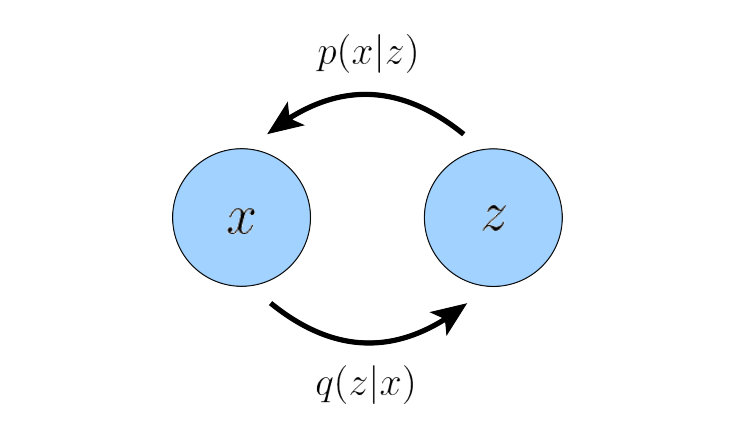
\includegraphics[width=5cm, height=3cm]{diffusion_1.png}
    \caption{VAE graphically represented}
    \end{figure}

\end{frame}


\begin{frame}{VAE}
    \begin{block}{Monte Carlo estimate}
        Encoder models multivatiate normal with diagonal covariance $q(z|x) \sim \mathcal{N}(\mu_{\phi}(x), \sigma^2_{\phi}(x)I)$, $p(z) \sim \mathcal{N}(0, I)$ 
        \[argmax_{\phi, \theta} \left(\mathbb{E}_{q_{\phi}(z|x)}\left[\log p_{\theta}(x|z)\right]  - D_{KL}(q_{\phi}
        (z|x) || p(z))\right)\]
        \[\approx argmax_{\phi, \theta} \left(\sum_{l=1}^L\log p_{\theta}(x|z^{(l)})  - D_{KL}(q_{\phi}(z|x) || p(z))\right)\]
        where latents ${z^{(l)}}_{l=1}^L$ are sampled from $q_{\phi}(z|x)$
    \end{block}
    \begin{block}{Reparametrization trick}
    $z \sim \mathcal{N}(\mu_{\phi}(x), \sigma^2_{\phi}(x)I)$ could be modeled as 
    \[z = \mu_{\phi}(x) + \sigma^2_{\phi}(x) \odot \varepsilon \text{ which } \varepsilon \sim \mathcal{N}(0, I)\] 
    \end{block}
\end{frame}

\section{Hierarchical VAE}
\begin{frame}{Hierarchical VAE}
    \begin{block}{HVAE}
    Joint distribution and the posterior
    \[p(x, z_{1:T}) = p(z_t) p_{\theta}(x|z_1)\prod_{t=2}^T p_{\theta}(z_{t-1}|z_t)\]
    \[q_{\phi}(z_{1:T}|x) = q_{\phi}(z_1|x)\prod_{t=2}^Tq_{\phi}(z_t|z_{t-1})\]
    \end{block}
    \begin{figure}[h]
        \centering
        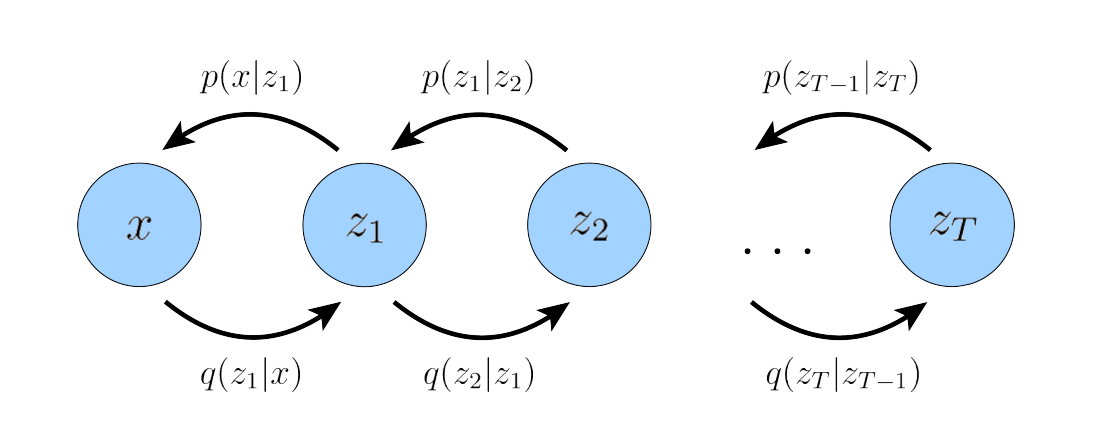
\includegraphics[width=5cm, height=2.3cm]{diffusion_2.png}
    \caption{Markovian Hierarchical Variational Autoencoder with T latents}
    \end{figure}
\end{frame}


\begin{frame}{Hierarchical VAE}
    \begin{block}{HVAE}
    During traning we also optimize ELBO
    \[\log p(x) \geq \mathbb{E}_{q_{\phi}(z_{1:T}|x)}\left[\dfrac{p(x, z_{1:t})}{q_{\phi}(z_{1:T}|x)}\right]\]
    \[\mathbb{E}_{q_{\phi}(z_{1:T}|x)}\left[\dfrac{p(z_t) p_{\theta}(x|z_1)\prod_{t=2}^T p_{\theta}(z_{t-1}|z_t)}{q_{\phi}(z_1|x)\prod_{t=2}^Tq_{\phi}(z_t|z_{t-1})}\right]\]
    \end{block}
    \begin{figure}[h]
        \centering
        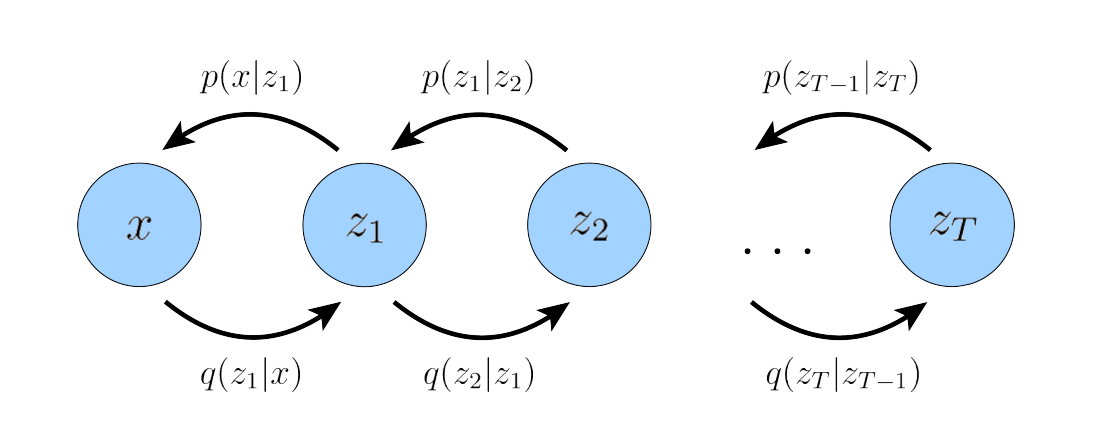
\includegraphics[width=5cm, height=2.3cm]{diffusion_2.png}
    \caption{Markovian Hierarchical Variational Autoencoder with T latents}
    \end{figure}
\end{frame}


\section{Variational Diffusion Models}
\begin{frame}{Variational Diffusion Models}
    \begin{block}{Similarities with HVAE}
    VDM is a Markovian HVAE with several restrictions
    \begin{itemize}
    \item Latent dimension is equal to data dimension
    \item Structure of each latent encoder is predefined as linear Gaussian model (not learned)
    \item Latent encoders are designed in such way that final latent $x_T$ is standard Gaussian
    \end{itemize}
    \end{block}
    \begin{figure}[h]
        \centering
        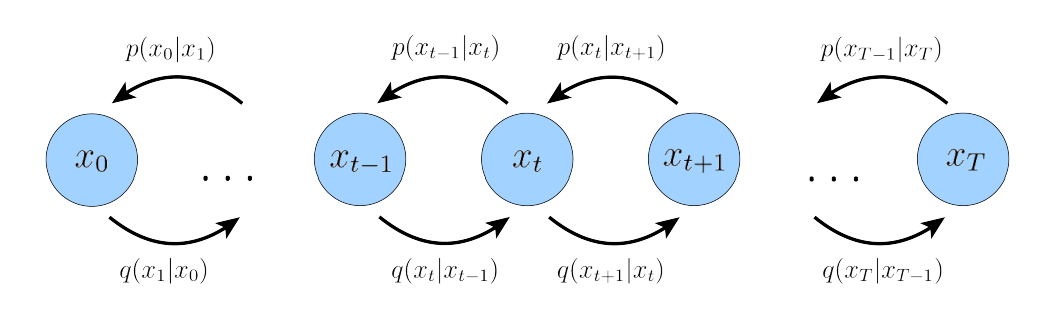
\includegraphics[width=7cm, height=2.3cm]{diffusion_3.png}
    \caption{A visual representation of a Variational Diffusion Model}
    \end{figure}
\end{frame}


\begin{frame}{Variational Diffusion Models}
    \begin{block}{Distributions}
    Latent variable posterior is same to MHVAE
    \[q(x_{1:T}|x_0) = \prod_{t=1}^T q(x_t|x_{t-1})\]
    Encoder transitions are denoted as Gaussian centered around previous latent
    \[q(x_t|x_{t-1}) = \mathcal{N}(x_t, \sqrt{\alpha_t}x_{t-1}, (1-\alpha_t)I)\]
    Last variable is a standard Gaussian 
    $x_T \sim \mathcal{N}(0, I)$.
    The joint distribution is
    \[p(x_{0:T}) = p(x_T) \prod_{t=1}^Tp_{\theta}(x_{t-1}|x_t)\]
    \end{block}
\end{frame}

\begin{frame}{Variational Diffusion Models}
    \begin{block}{Optimization}
    The VDM can be optimized by maximizing the ELBO
    \[\log p(x) = \log \int p(x_{0:T}) dx_{1:T}\]
    \[ \mathbb{E}_{q(x_1|x_0)}\left[ \log p_{\theta}(x_0|x_1)\right] - \mathbb{E}_{q(x_{T-1}|x_0)}D_{KL}\left(q(x_T|x_{T-1})||p(x_T)\right)\]
    \[-\sum_{t=1}^{T-1}\mathbb{E}_{q(x_{t-1}, x_{t+1}|x_0)} D_{KL}\left(q(x_t|x_{t-1}) || p_{\theta}(x_t|x_{t+1})\right)\]
    \end{block}
\end{frame}

\begin{frame}{Variational Diffusion Models}
    \begin{block}{Interpretation}
     Each term in ELBO could be interpreted as
    \begin{enumerate}
    \item Reconstruction term. Predicts the log probability of the data given first-step latent
    \item Prior matching term. Is minimized when the final latent distribution matches standard Gaussian prior
    \item Consistency term. A denosing step from a noisier image should match the corresponding noising step from a cleaner image
    \end{enumerate}
    \end{block}
    \begin{figure}[h]
        \centering
        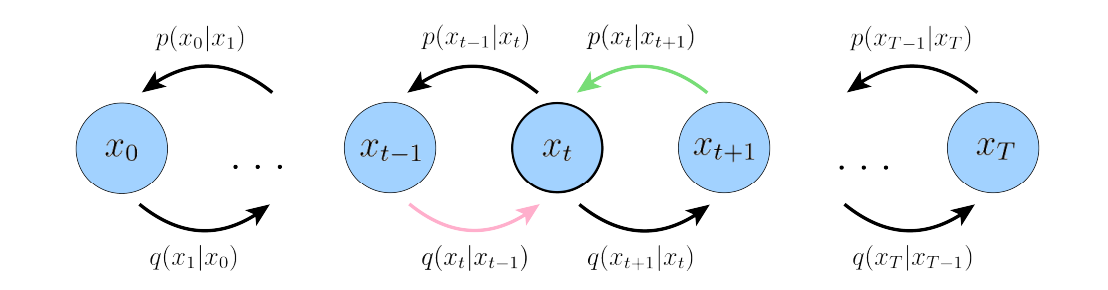
\includegraphics[width=7cm, height=2cm]{diffusion_4.png}
    \caption{A visual interpretation of ELBO}
    \end{figure}
\end{frame}

\begin{frame}{Variational Diffusion Models}
    \begin{block}{Rewriting ELBO}
    The consistency term is computed as an expectation over two random variance, so Monte Carlo estimation variance could be high.
    
    By Bayes rule:
    \[q(x_t|x_{t-1}, x_0) = \dfrac{q(x_{t-1}|x_t, x_0)q(x_t|x_0)}{q(x_{t-1}|x_0)}\]
    Let's rewrite ELBO so the expectation is taken only by one random variable
    
    Last term will be:
    \[-\sum_{t=2}^T \mathbb{E}_{q(x_t|x_0)} D_{KL}\left(q(x_{t-1}|x_t, x_0) || p_{\theta}(x_{t-1}|x_t)\right)\]
    Now we learn desired denoising transition step as an approxiamtion of ground-truth denoising transition step
    \end{block}
\end{frame}

\begin{frame}{Variational Diffusion Models}
    \begin{figure}[h]
    \centering
    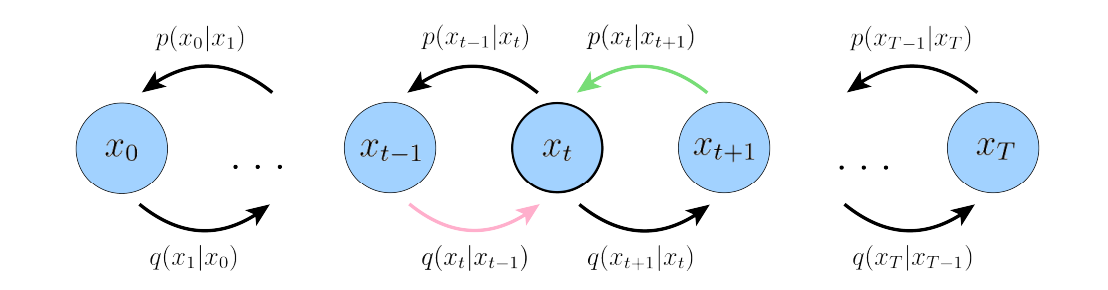
\includegraphics[width=7cm, height=2cm]{diffusion_4.png}
    \caption{Visual interpretation of ELBO with consistency term}
    \end{figure}
    \begin{figure}[h]
    \centering
    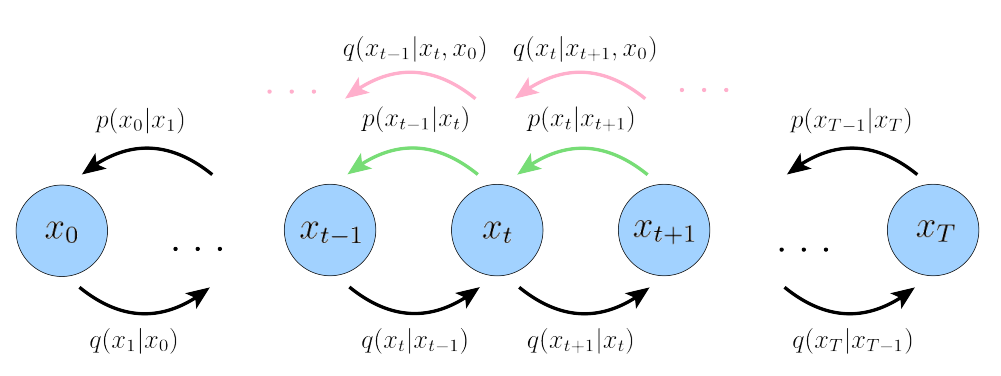
\includegraphics[width=7cm, height=2.7cm]{diffusion_5.png}
    \caption{Visual interpretation of ELBO with denoising matching term}
    \end{figure}
\end{frame}

\begin{frame}{Variational Diffusion Models}
    \begin{block}{Denoising term distributions}
    Each KL Divergence term ($D_{KL}\left(q(x_{t-1}|x_t, x_0) || p_{\theta(x_{t-1}|x_t)}\right)$) in the sum of denoising matching term is hardly to optimize for complex distributions.

    Bayes rule again
    \[q(x_{t-1}|x_t, x_0) = \dfrac{q(x_t|x_{t-1}, x_0)q(x_{t-1}|x_0)}{q(x_{t-1}|x_0)}\]
    Distribution of each component
    \[q(x_t|x_{t-1}, x_0) = q(x_t|x_{t-1}) = \mathcal{N}(x_t, \sqrt{\alpha_t}x_{t-1}, (1-\alpha_t)I)\]
    Also
    \[x_t = \sqrt{\alpha_t}x_{t-1} + \sqrt{1 - \alpha_t}\]
    So
    \[x_t \sim \mathcal{N}\left(\sqrt{\overline\alpha_t}, (1 - \overline\alpha_t)I\right)\]
    \end{block}
\end{frame}

\begin{frame}{Variational Diffusion Models}
    \begin{block}{Denoising term distributions}
    Using previous equations we can derive $q(x_{t-1}|x_t, x_0)$ $\sim \mathcal{N}\left(\mu_q(x_t, x_0), \Sigma_q(t)\right)$.
    Where
    \[\mu_q(x_t, x_0) = \dfrac{\sqrt{\alpha_t}(1 - \overline{\alpha}_{t-1})x_t + \sqrt{\overline{\alpha}_{t-1}}(1 - \alpha_t)x_0}{1 - \overline{\alpha_t}}\]
    \[\Sigma_q(t) = \frac{\sqrt{\overline{\alpha}_{t-1}}(1 - \alpha_t)x_0}{1 - \overline{\alpha_t}}, \dfrac{(1 - \alpha_t)(1 - \overline{\alpha}_{t-1})}{1 - \overline{\alpha}_{t}}\]
    \end{block}
    \begin{block}{Optimizing denoising matching term}
    We can also model denoising transition distribution $p_{\theta}(x_{t-1}|x_t)$ as Gaussian
    As all $\alpha$ are fixed, variance of denoiser should also be
    \[\Sigma_p(t) = \Sigma_q(t) = \sigma^2_q(t) I\]
    \[argmin_{\theta} D_{KL}(q(x_{t-1}|x_t, x_0) || p_{\theta}(x_{t-1}|x_t))\]
    \end{block}
\end{frame}

\begin{frame}{Variational Diffusion Models}
    \begin{block}{Optimizing denoising matching term}
    Furthermore
    \[argmin_{\theta} D_{KL}(q(x_{t-1}|x_t, x_0) || p_{\theta}(x_{t-1}|x_t))\]
    \[= argmin_{\theta} D_{KL} \left(\mathcal{N}(x_{t-1}, \mu_q, \Sigma_q(t)) || \mathcal{N}(x_{t-1}, \mu_{\theta}, \Sigma_q(t))\right)\]
    \[= argmin_{\theta} \dfrac{1}{2\sigma^2_q(t)}\left[\norm{\mu_{\theta}-\mu_q}_2^2\right]\]
    Using definition of $\mu_q$
     \[\mu_q(x_t, x_0) = \dfrac{\sqrt{\alpha_t}(1 - \overline{\alpha}_{t-1})x_t + \sqrt{\overline{\alpha}_{t-1}}(1 - \alpha_t)x_0}{1 - \overline{\alpha_t}}\]
     We can match $\mu_{\theta}$ to it closely by setting it 
     \[\mu_{\theta}(x_t, x_0) = \dfrac{\sqrt{\alpha_t}(1 - \overline{\alpha}_{t-1})x_t + \sqrt{\overline{\alpha}_{t-1}}(1 - \alpha_t)\widehat{x}_\theta(x_t, t)}{1 - \overline{\alpha_t}}\]
    \end{block}
\end{frame}

\begin{frame}{Variational Diffusion Models}
    \begin{block}{Optimizing denoising matching term}
    Thus, the optimization problem simplifies to
    \[argmin_{\theta} D_{KL}(q(x_{t-1}|x_t, x_0) || p_{\theta}(x_{t-1}|x_t))\]
    \[= argmin_{\theta} \dfrac{1}{2\sigma^2_q(t)} \dfrac{\overline{\alpha}_t (1 - \alpha_t)^2}{(1 - \overline{\alpha}_t)^2}{}\left[\norm{\widehat{x}_\theta(x_t, t)-x_0}_2^2\right]\]
    Therefore, optimizing a VDM boils down to learning a neural network to predict the original ground truth
    image from a noisified version of it.
    \end{block}
\end{frame}

\section{Equivalent interpretations of diffusion}
\begin{frame}{Equivalent interpretations of diffusion}
    \begin{block}{Reparametrization trick}
    \[x_0 = \frac{x_t - \sqrt{1 - \overline{\alpha}_t}\varepsilon_0}{\sqrt{\overline{\alpha}_t}}\]
    Where $\varepsilon_0 \sim \mathcal{N}(0, I)$ 
    
    Therefore, denoising transition mean:
    \[\mu_{\theta}(x_t, t) = \dfrac{1}{\sqrt{\alpha}_t}x_t - \dfrac{1 - \alpha}{\sqrt{1 - \overline{\alpha}_t}\sqrt{\alpha_t}}\widehat{\varepsilon}_{\theta}(x_t, t)\]
    Optimization problem:
    \[argmin_{\theta} \dfrac{1}{2\sigma^2_q(t)} \dfrac{\overline{\alpha}_t (1 - \alpha_t)^2}{(1 - \overline{\alpha}_t)^2}{}\left[\norm{\widehat{\varepsilon}_\theta(x_t, t)-x_0}_2^2\right]\]
    Where $\widehat{\varepsilon}_\theta(x_t, t)$ is a neural network that learns to predict noise
    \end{block}
\end{frame}

\begin{frame}{Equivalent interpretations of diffusion}
    \begin{block}{Tweedie's Formula}
    The true mean of an exponential family distribution, given samples drawn from it, can be estimated by the maximum likelihood estimate of the samples plus some correction term
    \[\mathbb{E}[\mu_z|z] = z + \sum_z \nabla{\log p(z)}\]
    Where $z \sim \mathcal{N}(\mu_z, \Sigma_z)$
    \end{block}
    \begin{block}{Our case}
    In our case
    \[q(x_t|x_0) \sim \mathcal{N}(\sqrt{\overline{\alpha}_t} x_0, (1 - \overline{\alpha}_t)I\]
    By Tweedie's formula
    \[\mathbb{E}[\mu_{x_t}|x_t] = x_t + (1 - \overline{\alpha}_t) \nabla_{x_t}{\log p(x_t)}\]
    \end{block}
\end{frame}

\begin{frame}{Equivalent interpretations of diffusion}
    \begin{block}{Our case}
    However, we know exact form of $\mu_{x_t} = \sqrt{\overline{\alpha}_t}$.
    Thus, we could derive
    \[\mu_q(x_t, x_0) = \dfrac{1}{\sqrt{\alpha_t}} x_t + \dfrac{1 - \alpha_t}{\sqrt{\alpha_t}}\nabla_{x_t}{\log p(x_t)}\]
    Approximation:
    \[\mu_{\theta}(x_t, t) = \dfrac{1}{\sqrt{\alpha_t}} x_t + \dfrac{1 - \alpha_t}{\sqrt{\alpha_t}}s_{\theta}(x_t, t)\]
    Optimization:
     \[argmin_{\theta} \dfrac{1}{2\sigma^2_q(t)} \dfrac{(1 - \alpha_t)^2}{\alpha_t}\left[\norm{s_{\theta}(x_t, t)-\nabla_{x_t}{\log p(x_t)}}_2^2\right]\]
    \end{block}
    Here neural network learns to predict score function - gradient of the log likelihood 
\end{frame}


\section{Guidance}
\begin{frame}{Guidance}
\begin{block}{Conditioning}
Often our aim is not only to model $p(x)$, but to model it given some additional information ($p(x|y)$) (image-text DALL-E 2). The joint distribution could be rewritten as
\[p(x_{0:T}|y) = p(x_T) \prod_{t=1}^Tp_{\theta}(x_{t-1}|x_t, y)\]
For example, y could be a text encoding in image-text generation, or a low-resolution image to perform super-resolution on.

Thus, we are able to learn neural networks by predicting
\[\widehat{x}_\theta(x_t, t, y) \approx x_0\]
But a conditional diffusion model trained in this way may potentially learn to ignore any given conditioning information.
\end{block}
\end{frame}


\begin{frame}{Guidance}
\begin{block}{Classifier guidance}
Let's use score-based definition of a diffusion model. Our goal is to learn $\nabla_{x_t}{\log(p(x_t|y))}$. By Bayes rule:
\[\nabla{\log(p(x_t|y))} = \nabla{\log(p(x_t))} + \nabla{\log(p(y|x_t))}\]
Importance of the last term could be controlled:
\[\nabla{\log(p(x_t|y))} = \nabla{\log(p(x_t))} + \gamma\nabla{\log(p(y|x_t))}\]
Drawback - relies on separate model which must be complex enough to deal with noised inputs.
\end{block}
\end{frame}

\begin{frame}{Guidance}
\begin{block}{Classifier-Free guidance}
Let's rewrite the classifier term from classifier guidance
\[\nabla{\log(p(y|x_t))} = \nabla{\log(p(x_t|y))} - \nabla{\log(p(x_t))}\]
Thus
\[\nabla{\log(p(x_t|y))} = \nabla{\log(p(x_t))} + \gamma(\nabla{\log(p(x_t|y))} - \nabla{\log(p(x_t))})\]
\[=\nabla{\log(p(x_t))} + \gamma\nabla{\log(p(x_t|y))} - \gamma\nabla{\log(p(x_t))}\]
\[=\gamma\nabla{\log(p(x_t|y))} + \nabla{\log(p(x_t))}(1 - \gamma)\]
\end{block}
\end{frame}

\section{References}
\begin{frame}{References}
\href{https://arxiv.org/pdf/2208.11970.pdf}{Understanding Diffusion Models: A Unified Perspective; Calvin Luno; 2022}
\end{frame}

\end{document}
